\begin{fact}
	$\forall q \in \RR$,
	$\exists\kern1pt! p \in \RRsp$ tel que 
	$\ln p = q$.
\end{fact}


\begin{proof}
	Nous connaissons le tableau de variations de $\ln$, voir le \reffact{ln-tab-var}.
	De plus, 
	$\ln$ est continue sur $\RRsp$, car dérivable sur $\RRsp$ selon le \reffact{ln-der}.
	Pour conclure,
	il suffit d'appliquer le \tvi, voir le \reffact{tvi}.
\end{proof}


% ----------------------- %


\begin{defi}
	$\forall q \in \RR$, 
	l'unique solution de $\ln x = q$ est notée $\exp q$.
	%
	Ceci définit une fonction $\exp: \RR \to \RRsp$ nommée \focus{exponentielle}.
	%
	Notons que $\exp 0 = 1$.
\end{defi}


% ----------------------- %


\begin{fact}
	$\forall x \in \RR$, $\ln ( \exp x ) = x$,
	et
	$\forall x \in \RRsp$, $\exp ( \ln x ) = x$.
\end{fact}


\begin{proof}	
	Nous devons juste vérifier la 2\ieme\ identité.
	En appliquant $\ln ( \exp X ) = X$ à $X = \ln x$,
	nous obtenons $\ln \big( \exp ( \ln x ) \,\big) = \ln x$.
	Par injectivité de la fonction $\ln$, nous arrivons à $\exp ( \ln x ) = x$ comme souhaité.
\end{proof}


% ----------------------- %


\begin{fact} \label{exp-sym-ln}
	Soient $\setproba{L}$ et $\setproba{E}$ les représentations graphiques respectives des fonctions $\ln$ et $\exp$.
	%
	Les courbes $\setproba{L}$ et $\setproba{E}$ sont symétriques par rapport à la 1\iere\ bissectrice $\Delta: y = x$.
\end{fact}


\begin{proof}
	Considérons $A(a;\exp a) \in \setproba{E}$.
	Notant $b = \exp a$, nous savons que $a = \ln b$.
	Ceci amène à considérer $B(b;\ln b) \in \setproba{L}$,
	c'est-à-dire $B(\exp a;a)$.
	%
	Or,
	$A(x_A;y_A)$ et $B(y_A;x_A)$ sont symétriques par rapport à $\Delta$
	(coordonnées d'un milieu, et critère d'orthogonalité):
	voir le graphique ci-dessous.
%	\footnote{
%		De façon plus élémentaire, nous pourrions raisonner via les triangles visibles sur le graphique en justifiant qu'ils sont tous carrés.
%	}
	Réciproquement, il faut considérer $B(b;\ln b) \in \setproba{L}$.
	Ce cas se traite de façon similaire.

	\begin{center}
		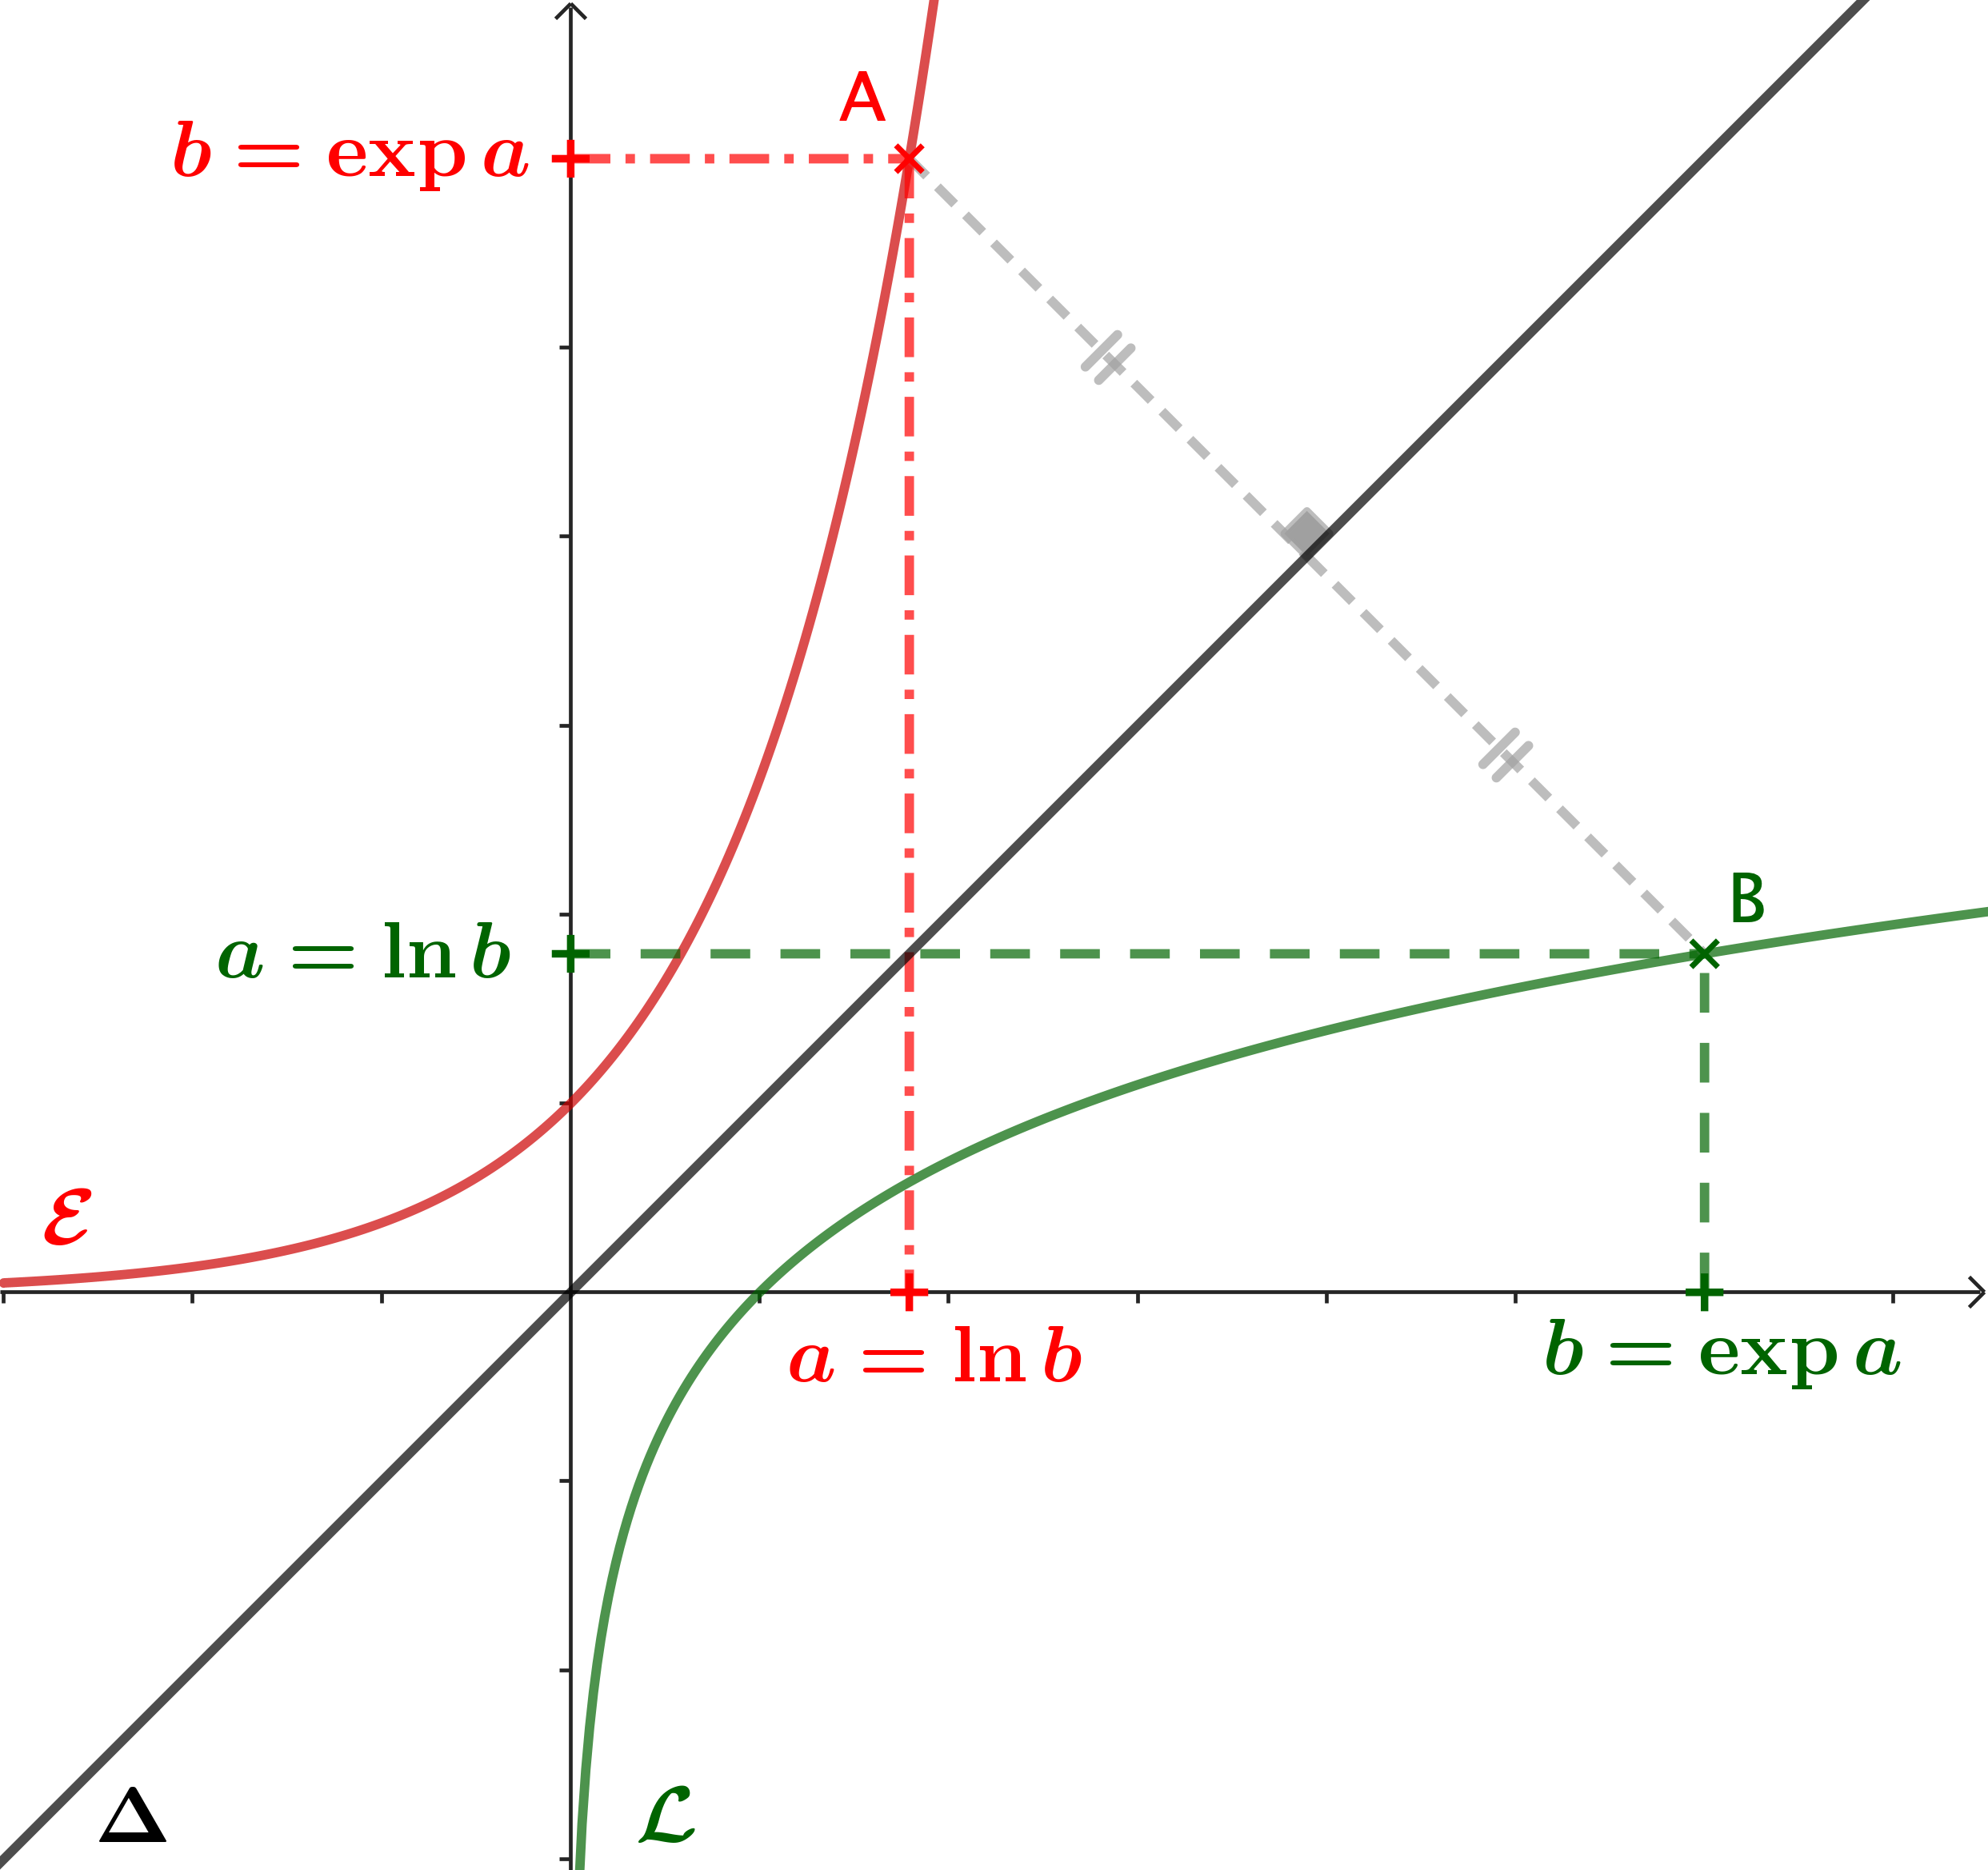
\includegraphics[scale=.85]{content/exp/graph.png}
	\end{center}
	
	\null
	\vspace{-6.5ex}
\end{proof}
